% -*- mode: latex; -*- mustache tags:  
\documentclass[10pt,twoside,english]{_support/latex/sbabook/sbabook}
\let\wholebook=\relax

\usepackage{import}
\subimport{_support/latex/}{common.tex}

%=================================================================
% Debug packages for page layout and overfull lines
% Remove the showtrims document option before printing
\ifshowtrims
  \usepackage{showframe}
  \usepackage[color=magenta,width=5mm]{_support/latex/overcolored}
\fi


% =================================================================
\title{Learning Object-Oriented Programming, Design and TDD with Pharo}
\author{Stéphane Ducasse}
\series{The Pharo TextBook Collection}

\hypersetup{
  pdftitle = {Learning Object-Oriented Programming, Design and TDD with Pharo},
  pdfauthor = {Stéphane Ducasse},
  pdfkeywords = {Introduction, programming, design, testing, Pharo, Smalltalk}
}


% =================================================================
\begin{document}

% Title page and colophon on verso
\maketitle
\pagestyle{titlingpage}
\thispagestyle{titlingpage} % \pagestyle does not work on the first one…

\cleartoverso
{\small

  Copyright 2017 by Stéphane Ducasse.

  The contents of this book are protected under the Creative Commons
  Attribution-ShareAlike 3.0 Unported license.

  You are \textbf{free}:
  \begin{itemize}
  \item to \textbf{Share}: to copy, distribute and transmit the work,
  \item to \textbf{Remix}: to adapt the work,
  \end{itemize}

  Under the following conditions:
  \begin{description}
  \item[Attribution.] You must attribute the work in the manner specified by the
    author or licensor (but not in any way that suggests that they endorse you
    or your use of the work).
  \item[Share Alike.] If you alter, transform, or build upon this work, you may
    distribute the resulting work only under the same, similar or a compatible
    license.
  \end{description}

  For any reuse or distribution, you must make clear to others the
  license terms of this work. The best way to do this is with a link to
  this web page: \\
  \url{http://creativecommons.org/licenses/by-sa/3.0/}

  Any of the above conditions can be waived if you get permission from
  the copyright holder. Nothing in this license impairs or restricts the
  author's moral rights.

  \begin{center}
    
\includegraphics[width=0.2\textwidth]{_support/latex/sbabook/CreativeCommons-BY-SA.pdf}
  \end{center}

  Your fair dealing and other rights are in no way affected by the
  above. This is a human-readable summary of the Legal Code (the full
  license): \\
  \url{http://creativecommons.org/licenses/by-sa/3.0/legalcode}

  \vfill

  % Publication info would go here (publisher, ISBN, cover design…)
  Layout and typography based on the \textcode{sbabook} \LaTeX{} class by Damien
  Pollet.
}


\frontmatter
\pagestyle{plain}

\tableofcontents*
\clearpage\listoffigures

\mainmatter

\chapter{A Digital Animal: A gluttonous Tamagotchi}
In this chapter we propose you to develop a small digital animal that has its own life and requires care from you. People were really fond of digital animals called tamagotchi. Therefore  we will build one step by step. This project is a pretext for revisiting the basic actions to define a class, instance variables, messages and methods. We will also discuss encapsulation.
\section{A gluttonous Tamagotchi}
We have to decide the behavior that our digital monster should have.
Here is the list of the behavior we propose you to implement for our  tamagoshi. 

\begin{itemize}
\item It can eat and digest food. It can be hungry when its tummy is empty and satisfied when it eats enough food.
\item It has its own life cycle with its own nights and days. It goes to sleep at night and wake up the morning.
\item It is gluttonous and selfish so falls asleep as soon as it eats enough.
\item Its change color depending on its mood.
\end{itemize}

We choose some colors to describe its state: 

\begin{itemize}
\item blue when it is satisfied possibly sleeping, 
\item black when sleeping but hungry, 
\item green when wakened up,
\item and red when it is hungry.
\end{itemize}
\section{Define Tamagotchi class}
Define a new package named for example 'Tamagotchi' and define the class \textcode{Tamagoshi}. As we would like to be able to interact with it and have a graphical representation, we define  the class \textcode{Tamagotchi} as a subclass of the class \textcode{Morph}. A morph is a graphical entity in Pharo. It knows how to draw itself on the screen. 

\begin{displaycode}{plain}
Morph subclass: #Tamagotchi
	instanceVariableNames: ''
	classVariableNames: ''
	package: 'Tamagoshi'
\end{displaycode}

We edit the class comment and write something in the vein of:

\begin{displaycode}{plain}
I represent a tamagotchi: A small virtual animal that has its own life.
\end{displaycode}

Executing the following snippet should get you a blue square as shown in \ref{squareTamagoshi}. Of course this is not really exciting but this is a start.

\begin{displaycode}{plain}
| t |
t := Tamagotchi new.
t openInHand
\end{displaycode}


\begin{figure}

\begin{center}
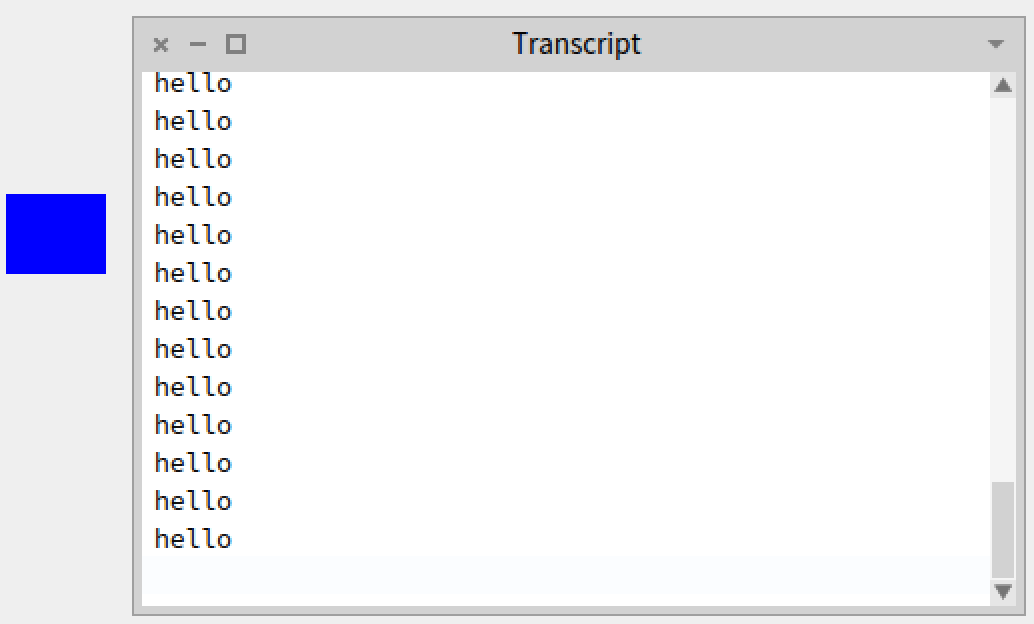
\includegraphics[width=0.5\textwidth]{/Users/ducasse/Workspace/FirstCircle/MyBooks/Bk-Writing/PharoBooks/LearningOOPWithPharoTrans/_result/pdf/Chapters/Tamagoshi/figures/tamagotchiAndHello.png}\caption{Our tamagotchi says hello in the Transcript. \label{squareTamagoshi}}\end{center}
\end{figure}

\subsection{Open a Transcript}
We will use the Transcript little window as a way to get some information from the tamagoshi. You can open a transcript using the tools menu or programmatically as follows:

\begin{displaycode}{plain}
Transcript open
\end{displaycode}

The method \textcode{step} of a morph is called by the system at regular interval.
We can redefine the method \textcode{step} of \textcode{Morph} as follows and we will obtain the situation depicted by Figure \ref{squareTamagoshi}.

\begin{displaycode}{plain}
Tamagoshi >> step
	"Print some information on the output"
	self logCr: 'hello'
\end{displaycode}

We should also define the interval between two steps, by defining the method \textcode{stepTime}.

\begin{displaycode}{plain}
Tamagotchi >> stepTime 
	"Return the time interval between two outputs"
	^ 500
\end{displaycode}
\section{Interacting with our live friend}
Before continuing any further, we want to show you some ways to interact with the tamagotchi.
\subsection{Halos}
Pharo offers little graphical menus called halos. To bring them, click and press option, command/control and shift.


\begin{figure}

\begin{center}
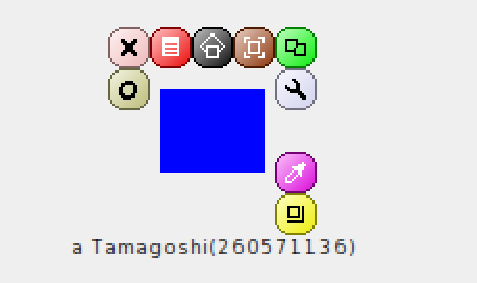
\includegraphics[width=0.5\textwidth]{/Users/ducasse/Workspace/FirstCircle/MyBooks/Bk-Writing/PharoBooks/LearningOOPWithPharoTrans/_result/pdf/Chapters/Tamagoshi/figures/TamaWithHalo.pdf}\caption{You can bring the halos around your tamagotchi by clicking on it while pressing option + command/control + shift \label{TamaWithHalo}}\end{center}
\end{figure}


With the halos you can 

\begin{itemize}
\item delete your tamagotchi. Pay attention you cannot bring it back.
\item move it
\item bring a menu and get an inspector as shown in Figure \ref{TamaWithInspectMenu}.
\end{itemize}


\begin{figure}

\begin{center}
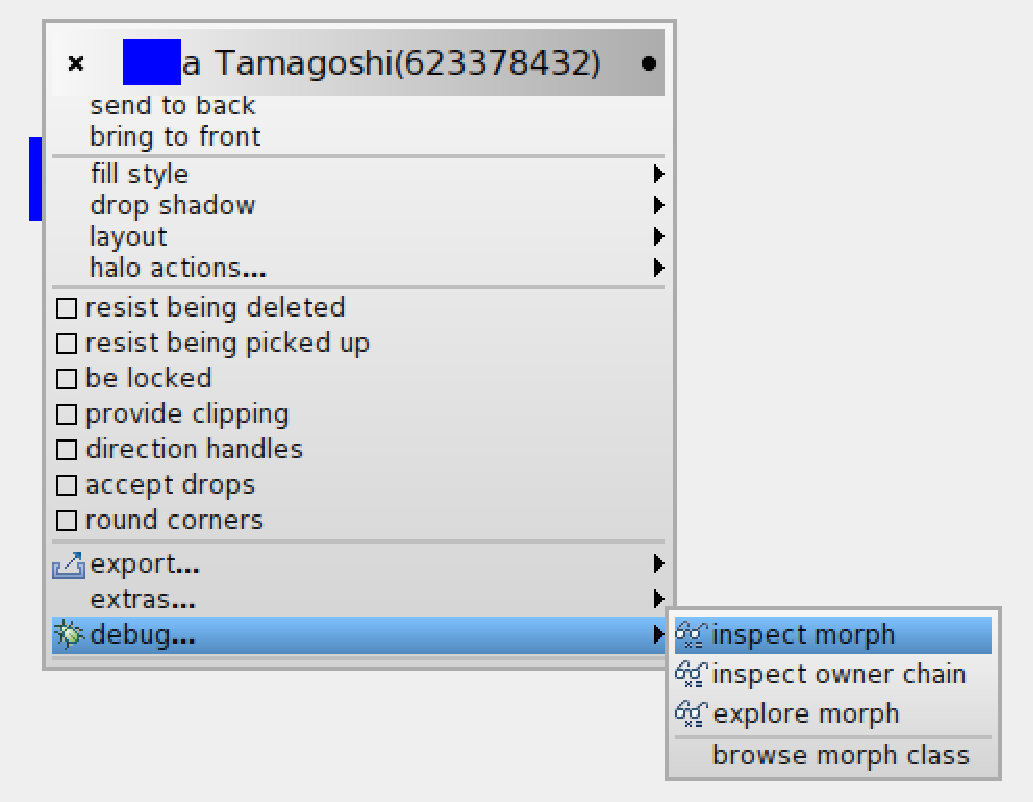
\includegraphics[width=0.5\textwidth]{/Users/ducasse/Workspace/FirstCircle/MyBooks/Bk-Writing/PharoBooks/LearningOOPWithPharoTrans/_result/pdf/Chapters/Tamagoshi/figures/TamaWithInspectMenu.pdf}\caption{Bringing an inspector to interact with a tamgotchi.\label{TamaWithInspectMenu}}\end{center}
\end{figure}


Note that it is easier to bring an inspector while creating the tamagotchi using the message \textcode{inspect} as follows:

\begin{displaycode}{plain}
| t |
t := Tamagotchi new.
t openInHand.
t inspect
\end{displaycode}
\subsection{Better use the playground}
You can also use the menu item do it and go of the playground to obtain an integrated inspector. In Figure \ref{TamaWithInspectorAndInstruction}. We created a tamagotchi and we selected \textbf{do it and go} and we ask the tamagotchi to display itself.  


\begin{figure}

\begin{center}
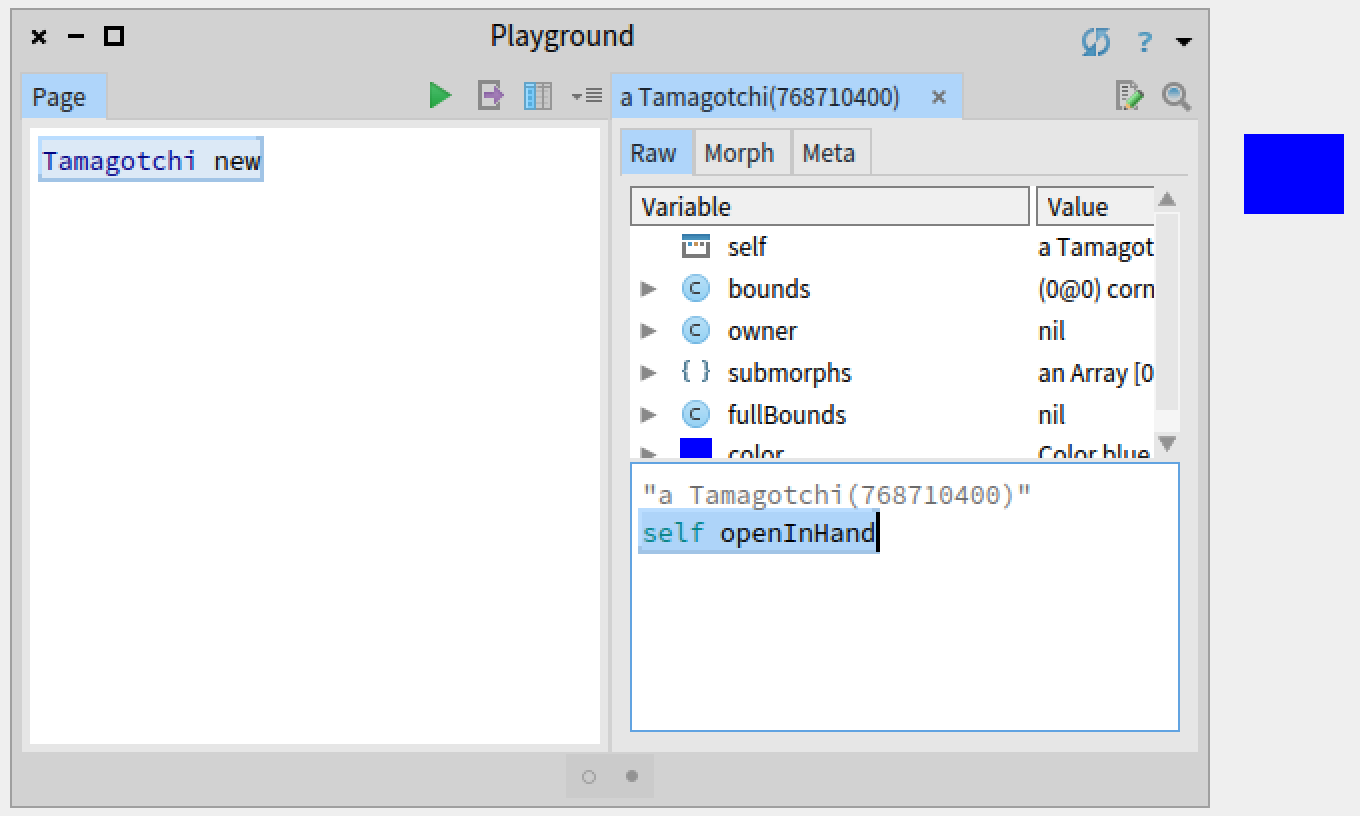
\includegraphics[width=1.0\textwidth]{/Users/ducasse/Workspace/FirstCircle/MyBooks/Bk-Writing/PharoBooks/LearningOOPWithPharoTrans/_result/pdf/Chapters/Tamagoshi/figures/TamaWithInspectorAndInstruction.png}\caption{Using Playground to get an inspector on a tamagotchi and sending it the message \textcode{openInHand}. \label{TamaWithInspectorAndInstruction}}\end{center}
\end{figure}

\section{Adding a Name}
\begin{displaycode}{plain}
Morph subclass: #Tamagoshi
	instanceVariableNames: 'name'
	classVariableNames: ''
	category: 'Tamagoshi'
\end{displaycode}

Make sure that if we do not give a name it is named \textcode{'pika'}.  When we create a new object by sending  the \textcode{new} message, the message \textcode{initialize} is sent. 
So we redefine it to put a new value with the string \textcode{'pika'}. We use the expression \textcode{super initialize} to make sure that the Morph is well initialized. This concept will be explained later in the book. 

\begin{displaycode}{plain}
Tamagotchi >> initialize
	super initialize. 
	name := 'pika'
\end{displaycode}

When we add a new instance variable to a class, all the existing instances get this instance variable but it will not be initialized correctly. So the best is to kill the tamagotchi and recreate one. You can kill a tamagotchi either using the halos or sending the message \textcode{delete} using the inspector. 


\begin{figure}

\begin{center}
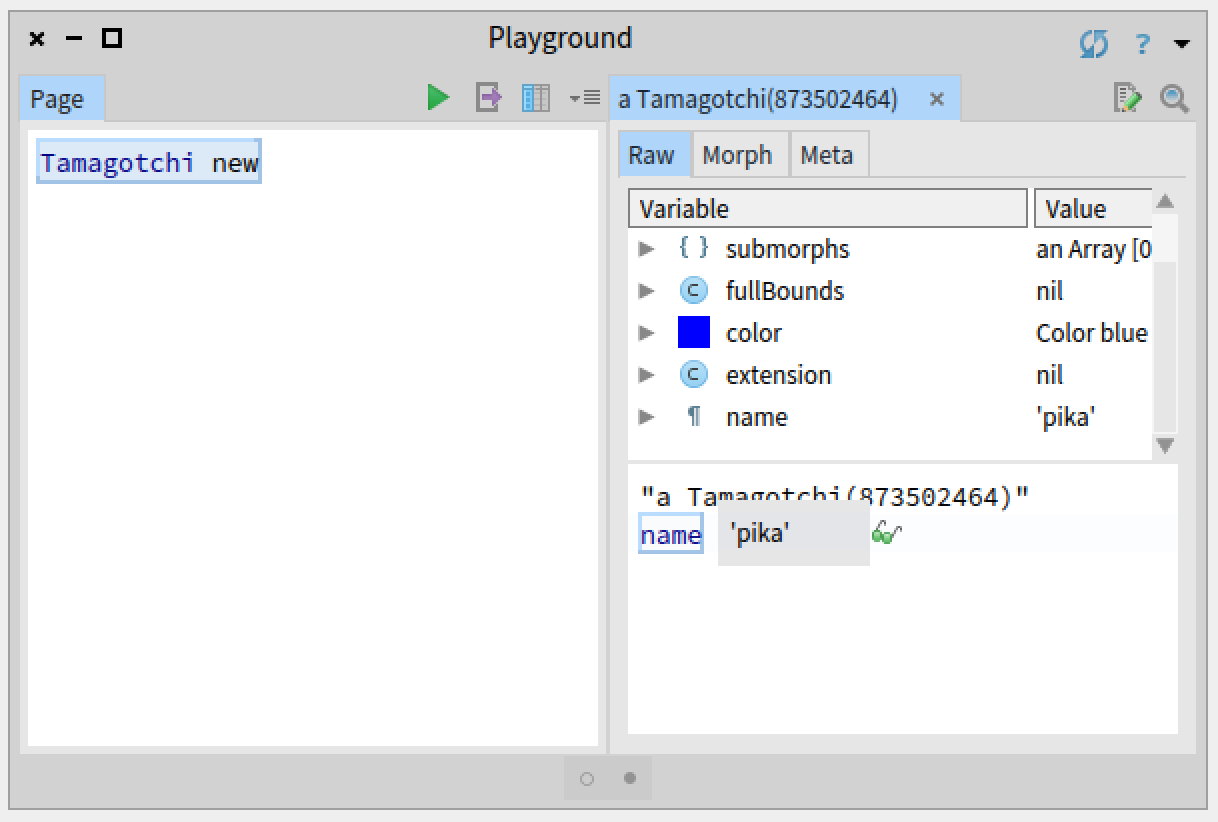
\includegraphics[width=0.5\textwidth]{/Users/ducasse/Workspace/FirstCircle/MyBooks/Bk-Writing/PharoBooks/LearningOOPWithPharoTrans/_result/pdf/Chapters/Tamagoshi/figures/TamaWithName.png}\caption{TamaWithName\label{TamaWithName}}\end{center}
\end{figure}



\begin{figure}

\begin{center}
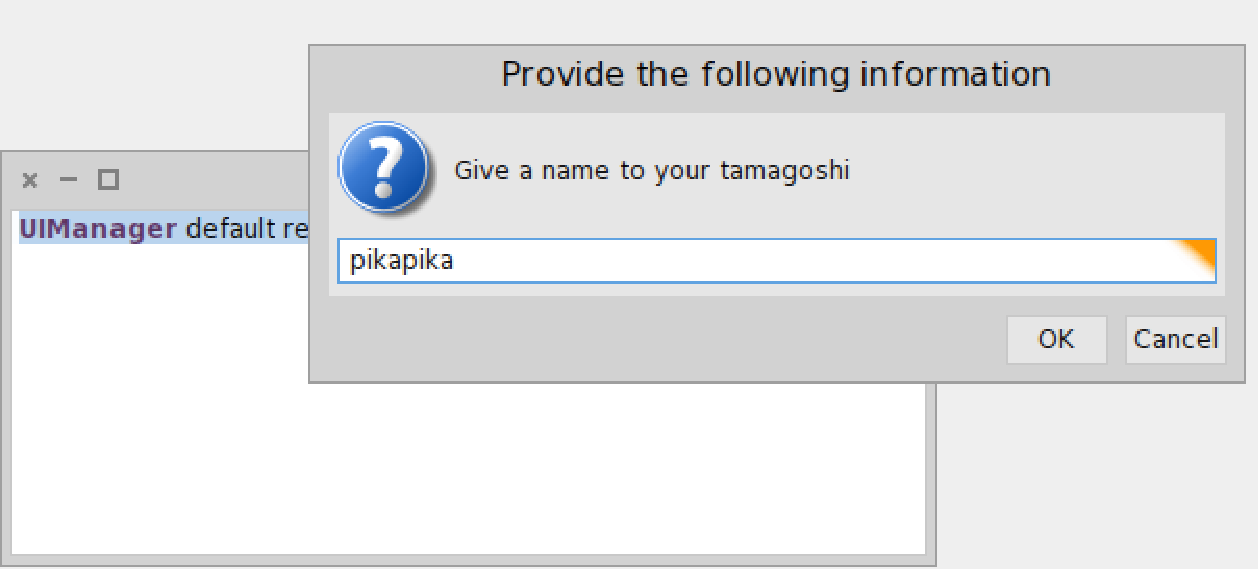
\includegraphics[width=0.5\textwidth]{/Users/ducasse/Workspace/FirstCircle/MyBooks/Bk-Writing/PharoBooks/LearningOOPWithPharoTrans/_result/pdf/Chapters/Tamagoshi/figures/withPopUp.pdf}\caption{withPopUp\label{withPopUp}}\end{center}
\end{figure}


\begin{displaycode}{plain}
UIManager default request:  'Give a name to your tamagoshi' 
\end{displaycode}


\begin{figure}

\begin{center}
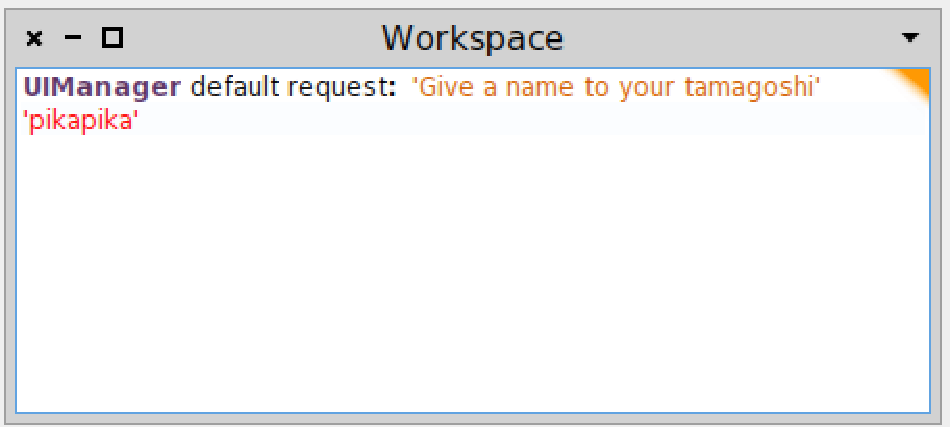
\includegraphics[width=0.5\textwidth]{/Users/ducasse/Workspace/FirstCircle/MyBooks/Bk-Writing/PharoBooks/LearningOOPWithPharoTrans/_result/pdf/Chapters/Tamagoshi/figures/requestInTranscript.pdf}\caption{requestInTranscript\label{requestInTranscript}}\end{center}
\end{figure}


\begin{displaycode}{plain}
Tamagotchi >> nameMe
	name := UIManager default request: 'Give a name please!'
\end{displaycode}

\begin{displaycode}{plain}
Tamagotchi >> step
	self logCr: 'hello, my name is ', name
\end{displaycode}


\begin{figure}

\begin{center}
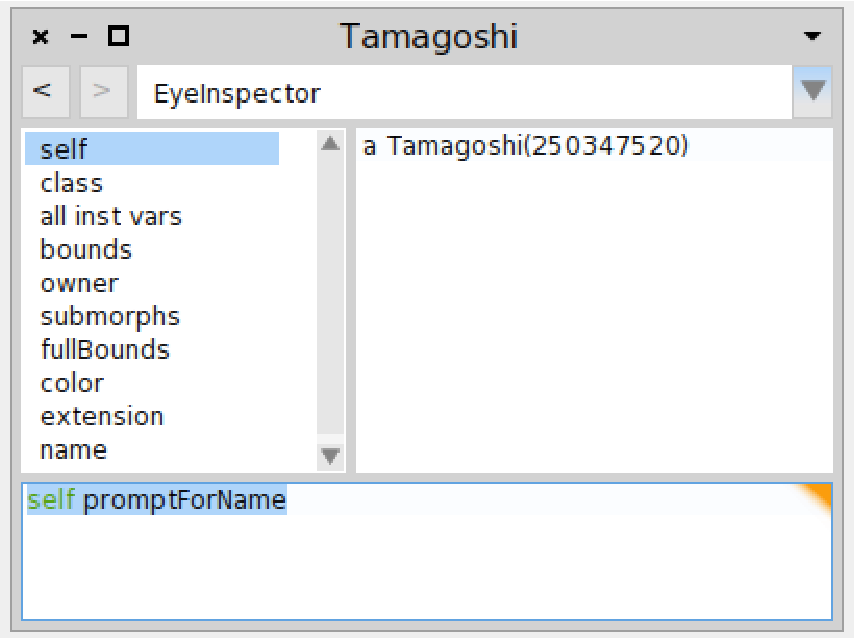
\includegraphics[width=0.5\textwidth]{/Users/ducasse/Workspace/FirstCircle/MyBooks/Bk-Writing/PharoBooks/LearningOOPWithPharoTrans/_result/pdf/Chapters/Tamagoshi/figures/inspectorWithFifiPrompt.pdf}\caption{inspectorWithFifiPrompt\label{inspectorWithFifiPrompt}}\end{center}
\end{figure}



\begin{figure}

\begin{center}
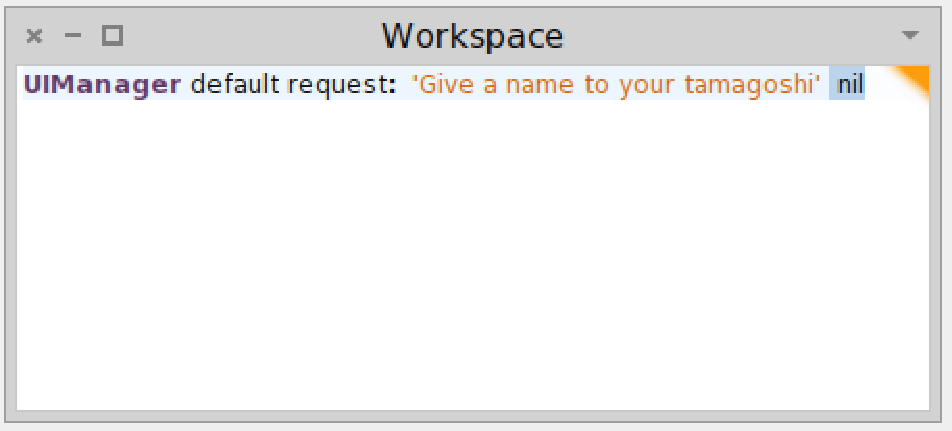
\includegraphics[width=0.5\textwidth]{/Users/ducasse/Workspace/FirstCircle/MyBooks/Bk-Writing/PharoBooks/LearningOOPWithPharoTrans/_result/pdf/Chapters/Tamagoshi/figures/promptWithNil.pdf}\caption{promptWithNil\label{promptWithNil}}\end{center}
\end{figure}

\section{Making nameMe more robust}
\begin{displaycode}{plain}
Tamagotchi >> nameMe

	| newName |
	newName := UIManager default request: 'Give a name please'.
	newName isNil 
		ifTrue: [ ]
		ifFalse: [ name := newName ]
\end{displaycode}

\begin{displaycode}{plain}
Tamagotchi >> nameMe

	| newName |
	newName := UIManager default request: 'Give a name please'.
	newName isNotNil 
		ifTrue: [ name := newName ]
\end{displaycode}
\section{Freeze}
\begin{displaycode}{plain}
Tamagotchi >> freeze
	"Freeze the behavior of the receiver until it receives the message unfreeze."
	self stopStepping
\end{displaycode}

\begin{displaycode}{plain}
Tamagotchi >> unfreeze
	"Get the receiver acting again."
	self startStepping
\end{displaycode}


\begin{figure}

\begin{center}
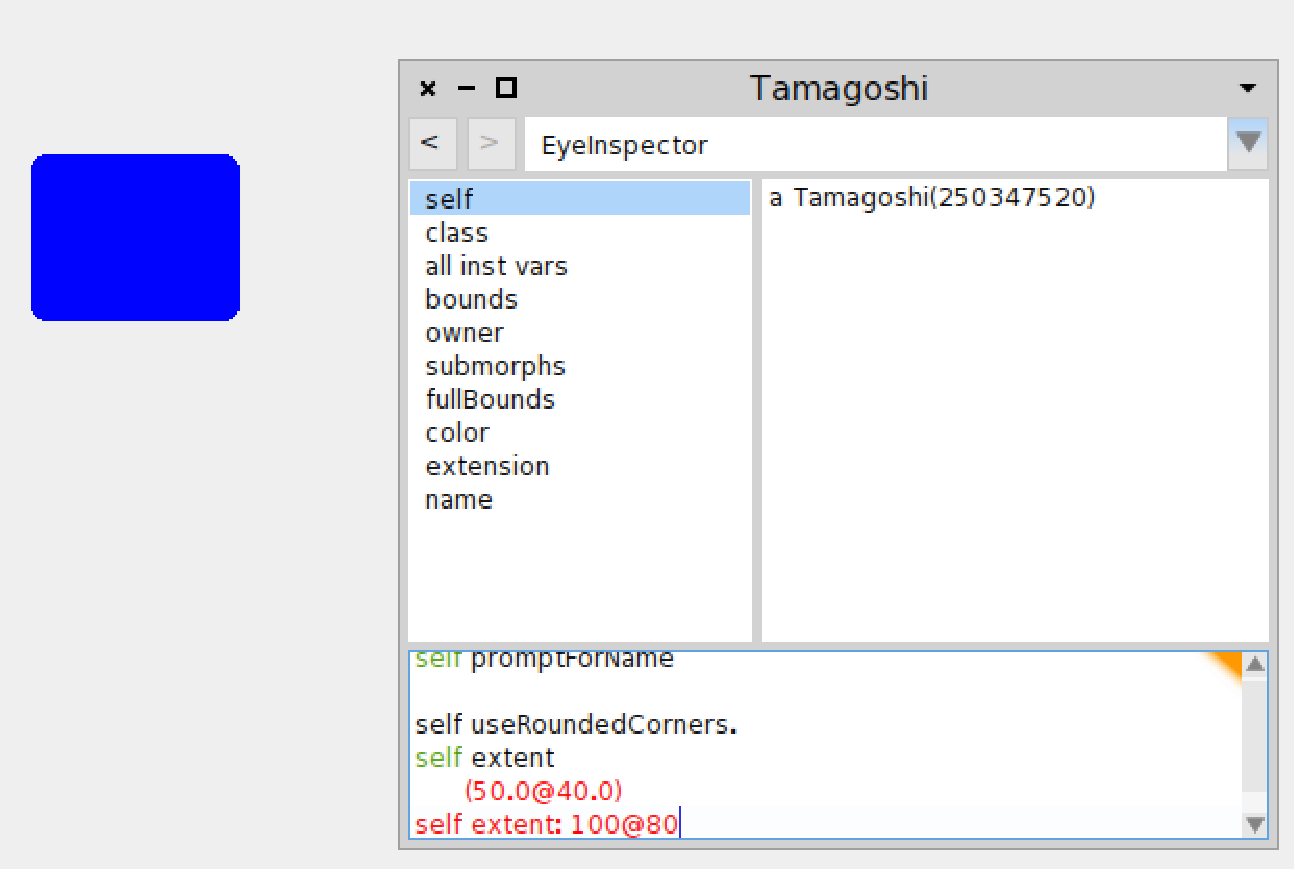
\includegraphics[width=0.5\textwidth]{/Users/ducasse/Workspace/FirstCircle/MyBooks/Bk-Writing/PharoBooks/LearningOOPWithPharoTrans/_result/pdf/Chapters/Tamagoshi/figures/LargerRounder.pdf}\caption{LargerRounder\label{LargerRounder}}\end{center}
\end{figure}


   \textcode{drawOn:} controls the drawing of the Morph. We can for example add an oval. 

\begin{displaycode}{plain}
drawOn: aCanvas

	super drawOn: aCanvas.
	aCanvas fillOval: self bounds
			fillStyle: self fillStyle 
			borderWidth: 3
			borderColor: Color white.
\end{displaycode}


\begin{figure}

\begin{center}
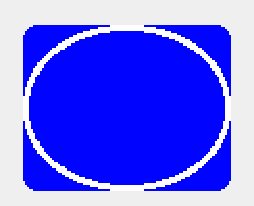
\includegraphics[width=0.5\textwidth]{/Users/ducasse/Workspace/FirstCircle/MyBooks/Bk-Writing/PharoBooks/LearningOOPWithPharoTrans/_result/pdf/Chapters/Tamagoshi/figures/WithEllipse.pdf}\caption{WithEllipse\label{WithEllipse}}\end{center}
\end{figure}


\begin{displaycode}{plain}
eyesOn: aCanvas

	| b m y |
	b := self bounds.
	m := b width / 2.
	y := b width / 4.
	aCanvas 
			fillOval: ((b origin   + (m - 20 @ y)) extent: 10@10)
			fillStyle: self fillStyle 
			borderWidth: 3
			borderColor: Color white.
	aCanvas 
			fillOval: ((b origin   + (m + 15 @ y)) extent: 10@10)
			fillStyle: self fillStyle 
			borderWidth: 3
			borderColor: Color white.
\end{displaycode}

\begin{displaycode}{plain}
drawOn: aCanvas

	super drawOn: aCanvas.
	self eyesOn: aCanvas
\end{displaycode}


\begin{figure}

\begin{center}
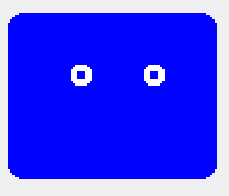
\includegraphics[width=0.5\textwidth]{/Users/ducasse/Workspace/FirstCircle/MyBooks/Bk-Writing/PharoBooks/LearningOOPWithPharoTrans/_result/pdf/Chapters/Tamagoshi/figures/justEyes.pdf}\caption{justEyes\label{justEyes}}\end{center}
\end{figure}


Now we can define the mouth of our digital animal by drawing two lines like in the following and we obtain Figure\textasciitilde{}ref\{fig:Smiling\}.

\begin{displaycode}{plain}
mouthOn: aCanvas

	| b m y middlePoint |
	b := self bounds.
	m := b width / 2.
	y := b width / 1.8.
	middlePoint := b origin +  ( m@y ).
	aCanvas 
		line: b origin + ((m-15) @ (y -5)) to:  middlePoint width: 3 color: Color black.
	aCanvas 
		line: b origin + ((m+15) @ (y -5)) to: middlePoint width: 3 color: Color black.
\end{displaycode}

\begin{displaycode}{plain}
drawOn: aCanvas

	super drawOn: aCanvas.
	self eyesOn: aCanvas.
	self mouthOn: aCanvas.
\end{displaycode}


\begin{figure}

\begin{center}
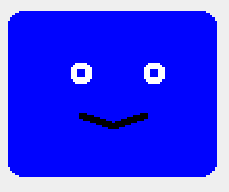
\includegraphics[width=0.5\textwidth]{/Users/ducasse/Workspace/FirstCircle/MyBooks/Bk-Writing/PharoBooks/LearningOOPWithPharoTrans/_result/pdf/Chapters/Tamagoshi/figures/Smiling.pdf}\caption{A smiling tamagoshi.\label{Smiling}}\end{center}
\end{figure}

\section{Eating Behavior}
Let us add a tummy to our tamagoshi. 

\begin{displaycode}{plain}
Morph subclass: #Tamagoshi
	instanceVariableNames: 'name tummy'
	classVariableNames: ''
	category: 'Tamagoshi'
\end{displaycode}

\begin{displaycode}{plain}
initialize

	super initialize. 
	self useRoundedCorners.
	self extent: 100@80.
	name := 'pika'.
	tummy := 5.
\end{displaycode}

Now we can also change the printing behavior to show its tummy.

\begin{displaycode}{plain}
step

	self logCr: 'hello, my name is ', name, ' and my tummy is: ', tummy printString.
\end{displaycode}

\begin{displaycode}{plain}
tummyOn: aCanvas
	aCanvas
		drawString: tummy printString
		at: self bounds corner - (20 @ 20)
		font: nil
		color: Color yellow
\end{displaycode}


\begin{figure}

\begin{center}
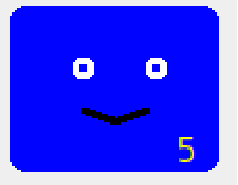
\includegraphics[width=0.5\textwidth]{/Users/ducasse/Workspace/FirstCircle/MyBooks/Bk-Writing/PharoBooks/LearningOOPWithPharoTrans/_result/pdf/Chapters/Tamagoshi/figures/withbBelly.pdf}\caption{withbBelly\label{withbBelly}}\end{center}
\end{figure}


do not forget to change the drawOn: method to invoke the tummyOn: method.

\begin{displaycode}{plain}
drawOn: aCanvas

	super drawOn: aCanvas.
	self eyesOn: aCanvas.
	self mouthOn: aCanvas.
	self tummyOn: aCanvas. 
\end{displaycode}

Now we would like to define the method eat so that we can feed our tamagoshi.

\begin{displaycode}{plain}
eat 

	tummy := tummy + 1
\end{displaycode}


\begin{figure}

\begin{center}
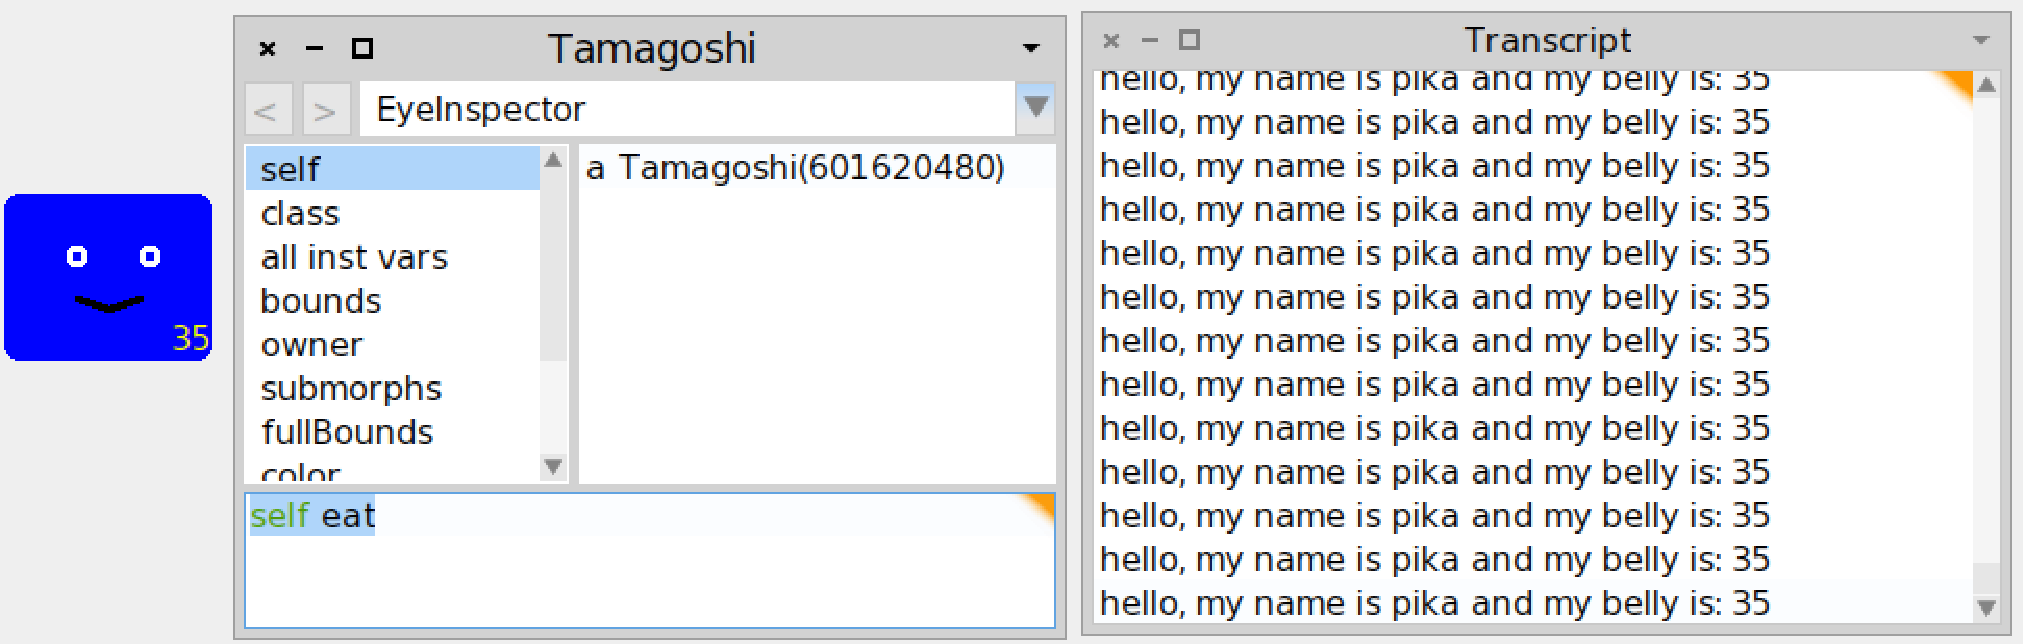
\includegraphics[width=0.5\textwidth]{/Users/ducasse/Workspace/FirstCircle/MyBooks/Bk-Writing/PharoBooks/LearningOOPWithPharoTrans/_result/pdf/Chapters/Tamagoshi/figures/eating.pdf}\caption{Now we show the food items in the tamagoshi' tummy\label{eating}}\end{center}
\end{figure}


\begin{displaycode}{plain}
eat 

	tummy := tummy + 1.
	self changed.
\end{displaycode}

Now we will tell the morph that it should react to mouse events.

\begin{displaycode}{plain}
handlesMouseDown: evt
	"Returning true means that the morph can react to mouse click"

	^ true
\end{displaycode}

And we will make sure that when we click on it, it gets fed.

\begin{displaycode}{plain}
mouseDown: evt
	
	self eat.	
\end{displaycode}

Now it may be wise to limit the stomach capability of our digital friend. We revise then the eat method to only increase it if we did not reach a limit. 

\begin{displaycode}{plain}
eat 

	tummy < 55
		ifTrue: [ tummy := tummy + 1
				  self changed]. 
\end{displaycode}
\section{Digesting}
Extract the code of the step method into a new method name talk.

\begin{displaycode}{plain}
talk

	self logCr: 'hello, my name is ', name, ' and my tummy is: ', tummy printString.
\end{displaycode}

\begin{displaycode}{plain}
step

	self talk.
\end{displaycode}

Now we are ready to make our tamagoshi digest its food. 

\begin{displaycode}{plain}
digest

	tummy := tummy - 1.
	self changed.
\end{displaycode}

Try with the inspector to send some digest messages to your tamagoshi. 

Now this is annoying to add the changed message everywhere so we introduce a method named: 

\begin{displaycode}{plain}
tummy: aNumber

	tummy := aNumber.
	self changed.
\end{displaycode}

and we use it in eat and digest

\begin{displaycode}{plain}
digest

	self tummy: tummy - 1.
\end{displaycode}

\begin{displaycode}{plain}
eat 

	tummy < 55
		ifTrue: [ self tummy: tummy + 1 ]. 
\end{displaycode}

\begin{displaycode}{plain}
step

	self talk.
	self digest.
\end{displaycode}

You will quickly see that digest is wrong because we will get negative numbers really fast. So first we change 
the definition of digest to be 

\begin{displaycode}{plain}
digest
	tummy = 0 
		ifFalse: [ self tummy: tummy - 1]
\end{displaycode}

Now since it is digesting too fast we should think how we could make our tamagoshi digest slower. What we need is 
a counter of the tick passed and based on that digest or not. So we add the hours instance variable to the class. 

\begin{displaycode}{plain}
Morph subclass: #Tamagoshi
	instanceVariableNames: 'name tummy hours'
	classVariableNames: ''
	category: 'Tamagoshi'
\end{displaycode}

\begin{displaycode}{plain}
initialize

	super initialize. 
	self useRoundedCorners.
	self extent: 100@80.
	name := 'pika'.
	tummy := 5.
	hours := 0.
\end{displaycode}

\begin{displaycode}{plain}
nextHour
	
	hours := hours + 1
\end{displaycode}

\begin{displaycode}{plain}
step

	self talk.
	self nextHour.
	self digest
\end{displaycode}

Now we can make our tamagoshi digest slower by simply making sure that several hours passed before it digests.
Just checking for example if the number of hours is divisible b a given number will do the trick.

\begin{displaycode}{plain}
step

	self talk.
	self nextHour.
	(hours isDivisibleBy: 3)
		ifTrue: [self digest ]
\end{displaycode}
\section{Hungry}
Now we get ready to make our tamagoshi changing face when he is hungry. 

\begin{displaycode}{plain}
isHungry

	^ tummy isZero
\end{displaycode}

We can now rewrite digest using isHungry as follow:

\begin{displaycode}{plain}
digest
	self isHungry
		ifFalse: [ self tummy: tummy - 1]
\end{displaycode}

\begin{displaycode}{plain}
hungryMouthOn: aCanvas

	| b m y middlePoint |
	b := self bounds.
	m := b width / 2.
	y := b width / 1.8.
	middlePoint := b origin +  ( m@y ).
	aCanvas 
		line: b origin + ((m-15) @ (y + 5)) to:  middlePoint width: 3 color: Color black.
	aCanvas 
		line: b origin + ((m+15) @ (y + 5)) to: middlePoint width: 3 color: Color black.
\end{displaycode}


\begin{figure}

\begin{center}
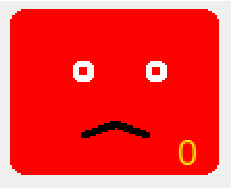
\includegraphics[width=0.5\textwidth]{/Users/ducasse/Workspace/FirstCircle/MyBooks/Bk-Writing/PharoBooks/LearningOOPWithPharoTrans/_result/pdf/Chapters/Tamagoshi/figures/hungry.pdf}\caption{Our tamagoshi shows now that he is hungry\label{hungry}}\end{center}
\end{figure}


Now we can change a bit the messages send by our tamagoshi. 

\begin{displaycode}{plain}
talk

	self isHungry
		ifTrue: [ self logCr: 'Please feed me' ]
		ifFalse: [ self logCr: 'hello, my name is ', name, ' and I''m ok'].
\end{displaycode}
\section{Nights and days}
Now we want to manage the night and day period of our tamagoshi. 

\begin{displaycode}{plain}
Morph subclass: #Tamagoshi
	instanceVariableNames: 'name tummy hours isNight'
	classVariableNames: ''
	category: 'Tamagoshi'
\end{displaycode}

\begin{displaycode}{plain}
initialize

	super initialize. 
	self useRoundedCorners.
	self extent: 100@80.
	name := 'pika'.
	tummy := 5.
	hours := 0.
	isNight := false
\end{displaycode}

\begin{displaycode}{plain}
isNight

	^ isNight
\end{displaycode}

\begin{displaycode}{plain}
switchDayPeriod
	"Switch from night to day and day to night"
	isNight := isNight not.
\end{displaycode}

\begin{displaycode}{plain}
checkAndNextDayPeriod
	"Switch from night to day and day to night when necessary" 

	(hours isDivisibleBy: 12)
		ifTrue: [ self switchDayPeriod ]
\end{displaycode}

We can change the messages to show that our animal is sleeping

\begin{displaycode}{plain}
talk
	self isNight
		ifTrue: [ self logCr: 'ZZZzzzzzzz' ]
		ifFalse: [ 
			self isHungry
				ifTrue: [ self logCr: 'Please feed me' ]
				ifFalse: [ self logCr: 'hello, my name is ' , name , ' and I''m ok' ] ]
\end{displaycode}

As we will see later, these conditionals all over the place are not that nice, each time we
add a new behavior we have to change talk and the drawOn: method logic becomes more and more complex. 

\begin{displaycode}{plain}
sleepyEyesOn: aCanvas

	| b m y |
	b := self bounds.
	m := b width / 2.
	y := b width / 4.
	aCanvas 
			fillOval: ((b origin   + (m - 20 @ y)) extent: 11@5)
			fillStyle: self fillStyle 
			borderWidth: 3
			borderColor: Color white.
	aCanvas 
			fillOval: ((b origin   + (m + 15 @ y)) extent: 11@5)
			fillStyle: self fillStyle 
			borderWidth: 3
			borderColor: Color white.
\end{displaycode}

\begin{displaycode}{plain}
drawOn: aCanvas
	super drawOn: aCanvas.
	self isNight
		ifTrue: [ 
				self sleepyEyesOn: aCanvas.
				self color: Color darkGray ]
		ifFalse: [ 
			self eyesOn: aCanvas.
			self isHungry
				ifTrue: [ 
					self color: Color red.
					self hungryMouthOn: aCanvas ]
				ifFalse: [ 
					self color: Color blue.
					self mouthOn: aCanvas ] ].
	self bellyOn: aCanvas.
	self changed.
\end{displaycode}


\begin{figure}

\begin{center}
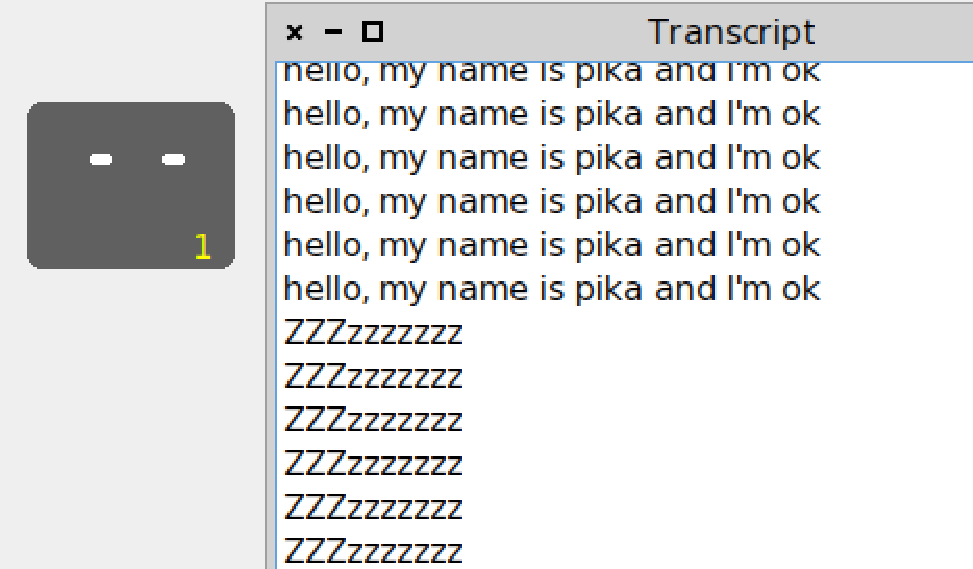
\includegraphics[width=0.5\textwidth]{/Users/ducasse/Workspace/FirstCircle/MyBooks/Bk-Writing/PharoBooks/LearningOOPWithPharoTrans/_result/pdf/Chapters/Tamagoshi/figures/sleeping.pdf}\caption{sleeping\label{sleeping}}\end{center}
\end{figure}

\section{Further Experiments}
Now we propose you different modifications to change the behavior of your tomagoshi. 

\begin{itemize}
\item Make that we can only feed the tomagoshi the day. 
\item Make it die when it is starving from too long time (hints you can use the method \textcode{delete} or \textcode{stopStepping}.
\item Make it happy, you could make it sings.
\item Change its graphical representation.  
\end{itemize}


% lulu requires an empty page at the end. That's why I'm using
% \backmatter here.
\backmatter

% Index would go here
\bibliographystyle{abbrv}
\bibliography{others.bib}
\end{document}
